% Define document class
\documentclass[twocolumn,twocolappendix]{aastex701}

\usepackage{graphicx}
\usepackage{xcolor}
\usepackage{amsmath}

% user-defined commands
\newcommand{\todo}[1]{{\color{red}#1}}
\newcommand{\osuaffil}{Department of Astronomy, The Ohio State University, 140 W. 18th Ave, Columbus OH 43210, USA}
\newcommand{\ccappaffil}{Center for Cosmology and AstroParticle Physics, The Ohio State University, 191 W. Woodruff Ave., Columbus OH 43210, USA}

\newcommand{\bracket}[2][H]{{\rm [#2/#1]}}
\newcommand{\kpc}{\,{\rm kpc}}
\newcommand{\Myr}{\,{\rm Myr}}
\newcommand{\Gyr}{\,{\rm Gyr}}
\newcommand{\dex}{\,{\rm dex}}
\newcommand{\Msun}{\,{\rm M}_\odot}
\newcommand{\kms}{\,{\rm km}\,{\rm s}^{-1}}

\shorttitle{What Makes the $[s/\alpha]$ Chemical Clock Tick?}
\shortauthors{Dubay et al.}

\begin{document}

% Title
\title{What Makes the $[s/\alpha]$ Chemical Clock Tick?}

\correspondingauthor{Liam Dubay}

% Author list
\author[0000-0003-3781-0747]{Liam O.\ Dubay}
\affiliation{\osuaffil}
\affiliation{\ccappaffil}
\email{dubay.11@osu.edu}
\author{co-authors}
\email{}
\affiliation{}

\begin{abstract}
    Abstract.
\end{abstract}

\section{Introduction}
\label{sec:introduction}

Stellar ages are a vital component of galactic archaeology studies. Recent years have seen an explosion of large stellar age catalogs that encompass a wide swath of the Milky Way. However, the most precise age estimation techniques, such as asteroseismology, are observationally expensive and apply to a limited range of stellar parameters. ``Chemical clocks,'' or empirically-calibrated relations between stellar age and atmospheric abundance ratios, promise reliable spectroscopic age estimates over a wider parameter space. The best-studied chemical clock is [C/N], which has a strong foundation in stellar physics but can only be used for stars on the red giant branch (RGB).

A number of studies have proposed the use of $[s/\alpha]$\textemdash the ratio of elements produced by the slow neutron-capture process to the $\alpha$-elements produced in core-collapse supernovae (CCSNe)\textemdash as a chemical clock. \citet{nissen_high-precision_2015} reported a tight correlation between [Y/Mg] and isochronal age for Solar twins and proposed its use as a sensitive chronometer. 

\begin{itemize}
    \item $[s/\alpha]$ correlates strongly with stellar age for a number of $s$-process elements \citep{casali_tracing_2025}.
    \item The [$s/\alpha$]--age relation may vary by region in the Galaxy \citep{ratcliffe_chemical_2024}, complicating its usefulness as an age indicator.
    \item The [$s/\alpha$]--age correlation is not theoretically justified---GCE models don't predict that the youngest stars have the highest [$s/\alpha$] \citep[e.g.,][]{grisoni_modelling_2020}.
\end{itemize}

Literature notes
\begin{itemize}
    \item \citet{edvardsson_chemical_1993} report a strong correlation between [Ba/H] and isochronal age.
    \item \citet{bensby_tracing_2007} find that [Ba/Fe] steadily increases over time for $\lesssim5\Gyr$ old thin disk stars (isochronal ages). They hypothesize that the flat trend with age for older stars is due to the $r$-process contribution.
    \item \citet{nissen_high-precision_2015} finds a tight correlation between [Y/Mg] and isochronal age for Solar twins (similar $\log g$, $T_{\rm eff}$, and [Fe/H]), and proposes its use as a chronometer. An abundance precision of 0.04 dex would correspond to an age precision of 1 Gyr.
    \item \citet{nissen_high-precision_2016} show correlations between [Y/Fe] and [Ba/Fe] with age for stars younger than 6 Gyr. They propose [Y/Mg] and [Y/Al] as chemical clocks.
    \item \citet{slumstrup_ymg_2017} find the [Y/Mg] relation holds for Solar-metallicity RC stars in four open clusters.
    \item \citet{feltzing_metallicity_2017} investigate the metallicity dependence of the [Y/Mg]--age correlation using abundances and isochronal ages from \citet{bensby_exploring_2014}. They find a strong dependence on metallicity, with stars at [Fe/H]$\approx-0.5$ showing a flat trend with age. They argue that this is due to the metallicity dependence of the Y yield: stars near Solar metallicity produce lots of first-peak elements (e.g., Sr, Y), while lower-metallicity stars instead produce more second-peak elements (e.g., Ba, La, Ce?).
\end{itemize}

Paper goals
\begin{itemize}
    \item Quantify the age--[$s/\alpha$] relation as a function of metallicity and Galactic position using SDSS-V. Is the relation universal or does it depend on other factors?
    \item Can GCE models match the age--[$s/\alpha$] relation? How much do we need to break yield predictions or enrichment timescales to do so?
\end{itemize}

\section{Observational Data}
\label{sec:data}

\begin{table*}
    \centering
    \caption{Sample selection parameters from MWM DR19 (see Section \ref{sec:data}).}
    \label{tab:sample}
    \begin{tabular}{lll}
        \hline\hline
        \multicolumn{1}{c}{Parameter} & \multicolumn{1}{c}{Range or Value} & \multicolumn{1}{c}{Notes} \\
        \hline
        $\log g$            & $[1.0, 3.5]$          & RGB selection \\
        $T_{\rm eff}$       & $[4000, 5500]$ K      & Recommended by \citet{meszaros_sdss-v_2025} \\
        $\bracket{M}$     & $>-1.5$               & Recommended by \citet{meszaros_sdss-v_2025} \\
        $S/N$               & $> 100$               & \todo{Justify} \\
        BAD flag            & 0                     & Bad flag for results\\
        SPECTRUM flag       & 0                     & Data reduction pipeline flags \\
        SDSS-IV EXTRATARG flag  & 0                 & Exclude stars outside main sample \\
        Mg, Fe, Ce flags    & 0                     & Abundances close to grid edges \\
        \hline
        Age training density    & $>3\times10^9$    & Recommended by \citet{stone-martinez_starflow_2025} \\
        \hline
    \end{tabular}
\end{table*}

We use data from the Milky Way Mapper (MWM; \todo{cite}), a program of the fifth generation of the Sloan Digital Sky Survey \citep[SDSS-V;][]{kollmeier_sdss-v_2017,kollmeier_sloan_2025} data release 19 \citep[DR19;][]{sdss_collaboration_nineteenth_2025}. The catalog includes all data from the previous Apache Point Observatory Galactic Evolution Experiment (APOGEE) DR17 \citep{abdurrouf_seventeenth_2022}. MWM DR19 data were obtained from the infrared APOGEE spectrographs \citep{wilson_apache_2019} mounted on the 2.5-meter Sloan Foundation Telescope \citep{gunn_25_2006} at Apache Point Observatory and the Ir{\'e}n{\'e}e DuPont Telescope \citep{bowen_optical_1973} at Las Campanas Observatory. 

Atmospheric parameters and chemical abundances were determined with the APOGEE Stellar Parameter and Chemical Abundance Pipeline \citep[ASPCAP;][]{garcia_perez_aspcap_2016}, which compares a grid of synthetic spectra \citep{hubeny_tlusty_2021} to the observed spectra using $\chi^2$ minimization. The line lists for most species are presented in \citet{smith_apogee_2021}, with additional Ce lines described by \citet{cunha_adding_2017}. All DR19 abundances assume local thermodynamic equilibrium (LTE). The spectral synthesis is further described by \citet{holtzman_apogee_2018} and \citet{jonsson_apogee_2020}.

We select red giant branch (RGB; $1.0<\log g<3.5$) stars with $S/N>100$. We limit our sample to the ``optimal region'' for Ce abundances, $T_{\rm eff}>4000$ K and $\bracket{M}>-1.5$, defined by \citet{meszaros_sdss-v_2025}. We further remove stars with the BAD flag, any APOGEE spectrum flags, and abundance flags for Mg, Fe, and Ce, as well as stars observed in SDSS-IV outside the main sample (EXTRATARG flag). This produces a primary sample of \todo{122,533} stars. The right-hand panel of Figure \ref{fig:kiel-diagram} plots a Kiel diagram of this sample, color-coded by [Ce/H]. A summary of our sample selection criteria is presented in Table \ref{tab:sample}.

\subsection{Kinematics}

The 6-D kinematic properties for stars in our sample are calculated using position, proper motion, parallax, and radial velocity measurements from {\it Gaia} DR3 \citep{gaia_collaboration_gaia_2023}. These coordinates are transformed into the Galactocentric cylindrical frame with {\tt astropy} \citep{astropy_collaboration_astropy_2013,astropy_collaboration_astropy_2018,astropy_collaboration_astropy_2022} using updated Solar position and motion parameters from \citet{hunt_multiple_2022}. Orbital parameters (such as the angular momentum $L_z$, energy $E$, guiding-center radius $R_g$, and maximum midplane distance $z_{\rm max}$) are calculated using the {\tt gala} package \citep{price-whelan_gala_2017} with the {\tt MilkyWayPotential2022} potential, assuming the circular velocity at the Solar position is $229\kms$ \citep{eilers_circular_2019}.

\begin{figure*}
    \centering
    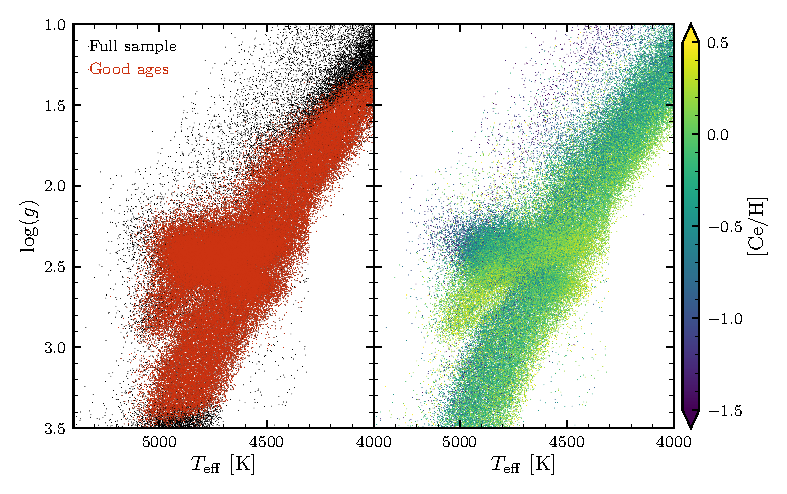
\includegraphics[width=0.8\textwidth]{figures/kiel_diagram.pdf}
    \caption{Kiel diagrams of our sample. {\it Left:} comparison between our full sample and the sample that exceeds the recommended age training density \citep{stone-martinez_starflow_2025}. {\it Right:} Kiel diagram of our full sample, color-coded by [Ce/H].}
    \label{fig:kiel-diagram}
\end{figure*}

\subsection{Stellar Ages}

We use the StarFlow \citep{stone-martinez_starflow_2025} catalog of stellar ages for MWM DR19. \citet{stone-martinez_starflow_2025} use a deep generative model trained on asteroseismic data to estimate ages for evolved stars. Their model retains information about the parameter space distribution of the training data and accounts for asymmetric uncertainties. We adopt their recommended training space density threshold of $>3\times10^9$, resulting in estimated ages for \todo{106,524} stars between \todo{$-1.05\lesssim\bracket{Fe}\lesssim+0.5$}. The left-hand panel of Figure \ref{fig:kiel-diagram} compares the Kiel diagram of this stellar age sample against our full sample.

\subsection{Cerium Abundance Precision}

\citet{meszaros_sdss-v_2025} estimated that the ASPCAP parameters for giant stars in DR19 have a precision of $50-90$ K for $T_{\rm eff}$, $0.07-0.09\dex$ for $\log g$, and $0.02-0.04\dex$ for metallicity, $\alpha$, and Mg. Due to the weak lines, Ce is less precisely measured. \citet{meszaros_sdss-v_2025} estimate an uncertainty in [Ce/M] of $\approx0.23$ for the solar neighborhood, open clusters, and wide binaries.

Ce lines in APOGEE reported by \citet{cunha_adding_2017}.

\begin{itemize}
    \item Check the spectra for high-[Mg/H] and low-[Ce/Mg] stars.
    \item Discuss abundance artifacts.
\end{itemize}

\subsection{Corrective Abundance Offsets}

% Zero-point offsets
% DR17 (from allStarLite)
% Ce: -0.05566
% Mg: +0.063523
% Fe: 0
% DR19 (from allStar)
% Ce: +0.14872
% Mg: +0.004268
% Fe: +0.013549
% DR19 (from Meszaros++ 2025)
% Ce: -0.1186
% Mg: -0.00005
% Fe: ---
% Why are these different??

\todo{Contribution from Tawny.}

We divide our sample into high-Ia and low-Ia populations using the boundary condition
\begin{equation}
    \bracket[Mg]{Fe} = 
    \begin{cases}
        -0.09, & \bracket{Fe}>0 \\
        -0.09+0.13\times\bracket{Fe}, & \bracket{Fe}<0.
    \end{cases}
    \label{eq:alpha-cut}
\end{equation}
High-Ia stars lie above this boundary, while low-Ia stars lie below; we exclude stars within $\pm0.02\dex$ of this boundary from either population.

Figure \ref{fig:logg-calibrations} shows the effect of the corrective offsets on [Ce/Mg] and [Fe/Mg]. Across different $\log(g)$ bins, the uncorrected [Ce/Mg] trends with [Mg/H] vary by up to $\sim0.3\dex$ for high-Ia stars, and $\sim0.1\dex$ for low-Ia stars. The corrective offsets ensure that abundances are consistent across the full range of $\log(g)$ in the sample.

\begin{figure}
    \centering
    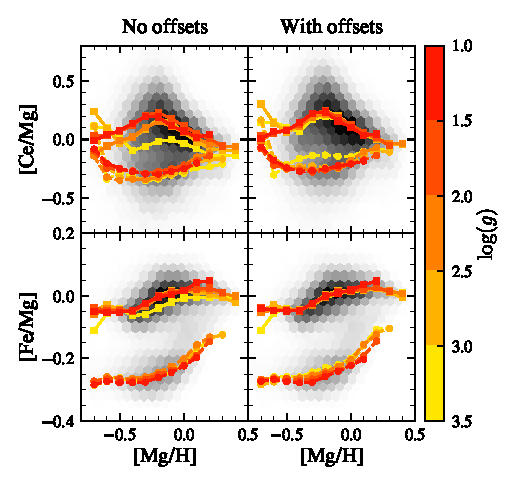
\includegraphics[width=\linewidth]{figures/logg_calibrations.pdf}
    \caption{Demonstration of corrective $\log(g)$ offsets applied to DR19 Ce and Fe abundances.}
    \label{fig:logg-calibrations}
\end{figure}

\subsection{Residual Abundances}

\section{Results}
\label{sec:results}

Outline:
\begin{itemize}
    \item We confirm the striking trend in the [Ce/Mg]--age relation, with the oldest stars having the lowest [Ce/Mg] and the youngest having the highest (Figures \ref{fig:cemg-mgh-age} and \ref{fig:dataset-comparison}).
    \item Comparison with other datasets shows our [Ce/Mg]--age relation is trustworthy (Figure \ref{fig:dataset-comparison}).
    \item Local age trends show a significant dependence on metallicity. Stars with slightly sub-Solar metallicity have the steepest trend, while metal-rich and metal-poor stars have shallow or flat trends (Figure \ref{fig:local-age-trends}). We calculate residual abundances to control for metallicity (Figure \ref{fig:residual-explainer}).
    \item The high-Ia population [Ce/Mg]--[Mg/H] trend varies by region of the Galaxy, while the low-Ia population is consistent across $R_{\rm guide}$ and $z_{\rm max}$ (Figure \ref{fig:median-trends-grid}).
    \item Similarly, the $\Delta\bracket{Ce}$--age trend varies by region for the high-Ia population. The slope is steepest in the outer galaxy, and the trend disappears in the inner galaxy (Figures \ref{fig:residual-abundances} and \ref{fig:median-age-trends}; pick one).
    \item The radial gradient evolves from negative to flat in [Ce/H], and flat to positive in [Ce/Mg], moving from older to younger populations. Low-Ia stars show a flat gradient and are $\sim0.5\dex$ lower in [Ce/H] and $\sim0.3\dex$ lower in [Ce/Mg] than high-Ia stars on average (Figure \ref{fig:ce-gradient}).
\end{itemize}

\todo{To do:
\begin{itemize}
    \item Can low-metallicity Ce abundances constrain [Ce/Mg] ``plateau'' (if it exists at all)?
    \item Compare SDSS-V trends to \citet{casali_tracing_2025} trends.
    \item Is the break in the trend at $\sim6\Gyr$ important? (Figure \ref{fig:median-age-trends}).
    \item Discuss halo stars, accreted vs in-situ. How do trends compare vs local group galaxies? Make sure stars in our sample aren't in local dwarfs.
    \item Other kinematic info if useful
\end{itemize}
}

\begin{figure}
    \centering
    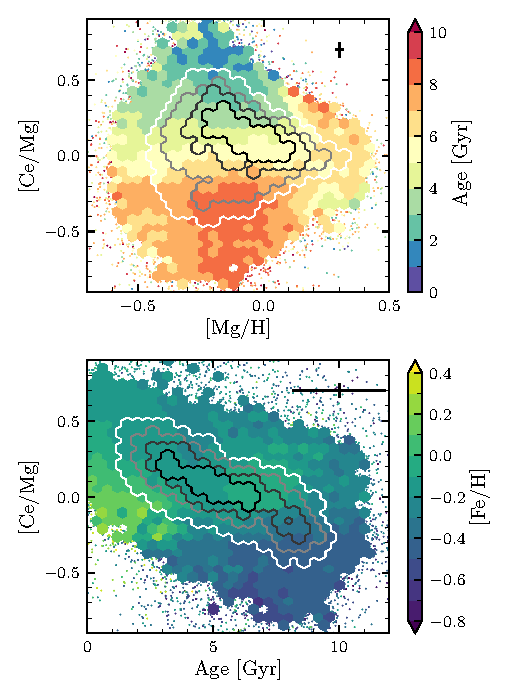
\includegraphics[width=\linewidth]{figures/cemg_mgh_age.pdf}
    \caption{The distribution of abundances in the [Ce/Mg]--[Mg/H] plane for our full sample, color-coded by the median stellar age. Each hexagonal bin contains a minimum of 10 stars; in lower-density regions, each star is plotted individually. The grayscale outlines represent linearly-spaced density contours, with the black contour encompassing the highest density of stars.}
    \label{fig:cemg-mgh-age}
\end{figure}

Figure \ref{fig:cemg-mgh-age} shows the median stellar age as a function of [Mg/H] and [Ce/Mg]. A broad age trend is immediately obvious: stars with low [Ce/Mg] are on average the oldest in the sample, while stars with high [Ce/Mg] are the youngest. Most of the old, low-[Ce/Mg] stars belong to the low-Ia population. Stars with Solar [Ce/Mg] are typically $\sim4-6\Gyr$ old, across a wide range of metallicity ($-0.5\lesssim\bracket{Mg}\lesssim+0.2$). The spread in [Ce/Mg] and age is broadest at $\bracket{Mg}\approx-0.2$, while the most Mg-rich stars occupy a narrow range of near-Solar [Ce/Mg] with median ages of $\sim6-7\Gyr$.

\subsection{Age Trend Validation}

\begin{figure}
    \centering
    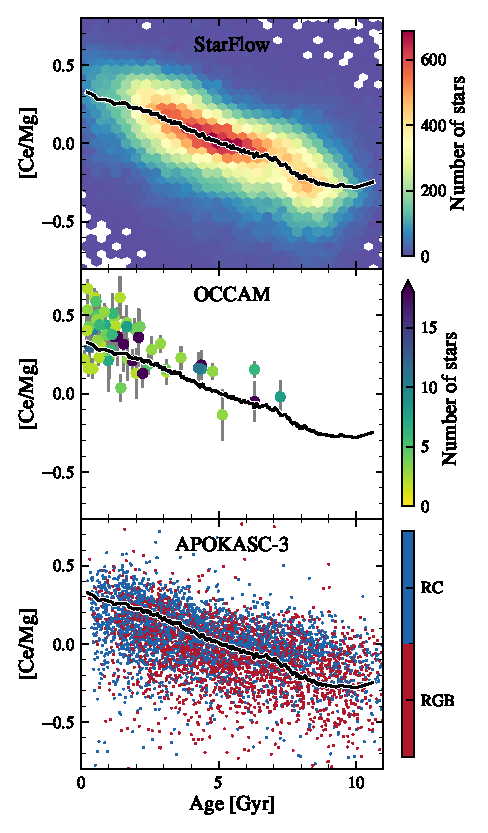
\includegraphics[width=\linewidth]{figures/dataset_comparison.pdf}
    \caption{Comparison of the age--[Ce/Mg] trend between MWM+StarFlow, APOKASC-3, and OCCAM. Each survey uses different age estimation techniques, but the abundances on the y-axis all come from DR19. For the sake of comparison, we do not apply $\log g$ corrections to the abundances in this plot.}
    \label{fig:dataset-comparison}
\end{figure}

Figure \ref{fig:dataset-comparison} compares the age--[Ce/Mg] relation from our sample against two other age catalogs: the Open Cluster Chemical Abundances and Mapping Survey \citet[OCCAM;][]{otto_open_2026} and the APOGEE-Kepler Asteroseismic Catalog \citep[APOKASC-3;][]{pinsonneault_apokasc-3_2025}. We use DR19 abundances for both catalogs. The OCCAM data include clusters with at least one RGB star with a measurement of [Ce/H]. Most of the clusters are young, $\lesssim2\Gyr$, and these clusters also show the largest spread in [Ce/Mg]. \todo{Still, the OCCAM trend qualitatively agrees with our sample.} We also see agreement with the trend in the APOKASC-3 data, although this is not surprising because StarFlow is trained on APOKASC-3.

\subsection{Metallicity Dependence}

\begin{figure}
    \centering
    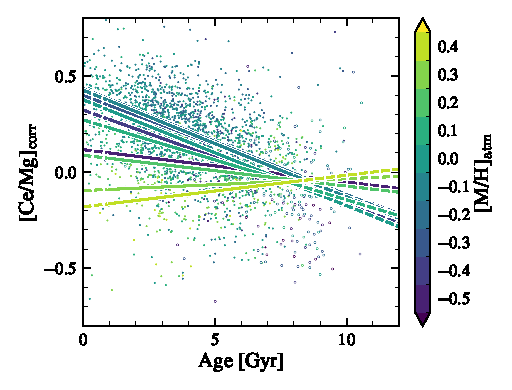
\includegraphics[width=\linewidth]{figures/local_age_trends.pdf}
    \caption{Solar neighborhood age--[Ce/Mg] relation and linear fits binned by metallicity.}
    \label{fig:local-age-trends}
\end{figure}

\begin{figure}
    \centering
    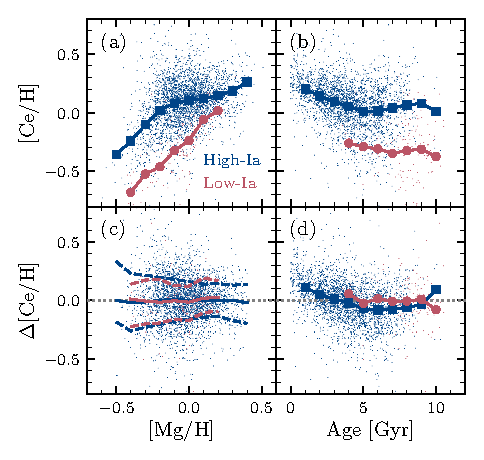
\includegraphics[width=\linewidth]{figures/residual_explainer.pdf}
    \caption{Demonstration of Ce residual abundance calculation. Top row: median trend in [Ce/H] as a function of [Mg/H] (left) and age (right) for the high- and low-Ia populations. Bottom row: median trend in $\Delta$[Ce/H] as a function of [Mg/H] (left) and age (right). Both populations show similar trends with age in [Ce/H] and $\Delta$[Ce/H].}
    \label{fig:residual-explainer}
\end{figure}

\subsection{Trends across the Galaxy}

\begin{figure*}
    \centering
    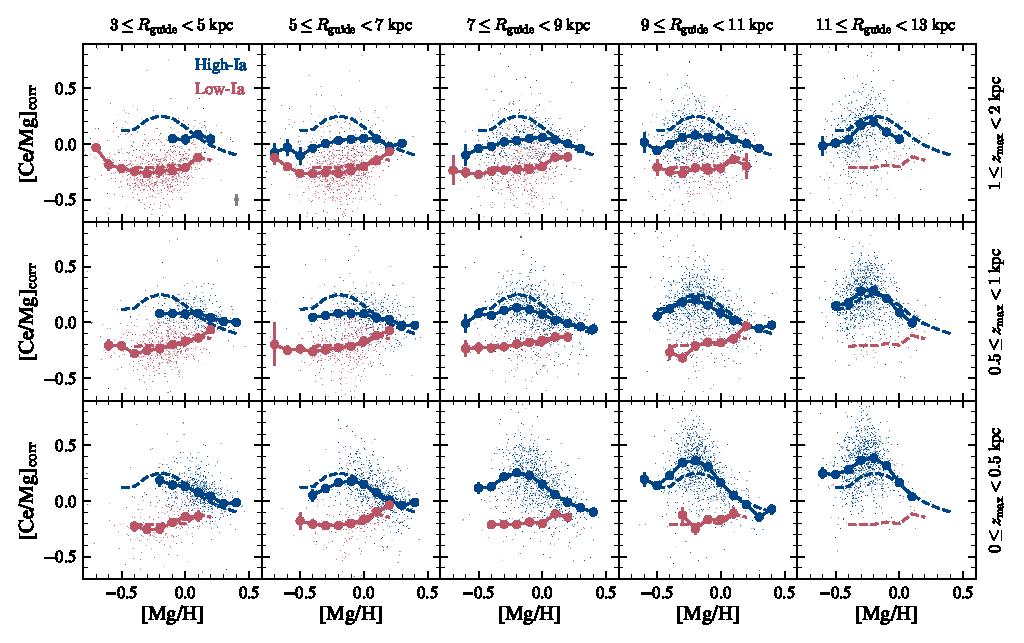
\includegraphics[width=\linewidth]{figures/median_trends_grid.pdf}
    \caption{The $\log(g)$-corrected [Ce/Mg] as a function of [Mg/H] for high- and low-Ia populations across the Galaxy. Each panel corresponds to a bin in $R_{\rm guide}$ (increasing left to right) and $z_{\rm max}$ (increasing bottom to top). The small blue (red) points plot individual abundances of high-Ia (low-Ia) stars. For visual clarity, only a random sample of 1,000 stars are plotted in each panel. The solid lines with large points plot the median [Ce/Mg] in bins of [Mg/H] for each region, and for reference the dashed lines indicate the median trends in the Solar neighborhood ($7\leq R_{\rm guide}<9\kpc$, $z_{\rm max}<0.5\kpc$). The gray error bars in the top left panel indicate the median abundance errors for the full DR19 sample.}
    \label{fig:median-trends-grid}
\end{figure*}

Figure \ref{fig:median-trends-grid} shows how the [Ce/Mg] median trend with [Mg/H] changes with position in the Galaxy. In the Solar neighborhood, the median high-Ia trend peaks at $\bracket{Mg}=-0.2$ with $\bracket[Mg]{Ce}\approx+0.25$, and the most metal-rich stars have lowest $\bracket[Mg]{Ce}\approx-0.1$. Moving from the inner to the outer Galaxy, the metallicity with the highest [Ce/Mg] 

% \begin{figure*}
%     \centering
%     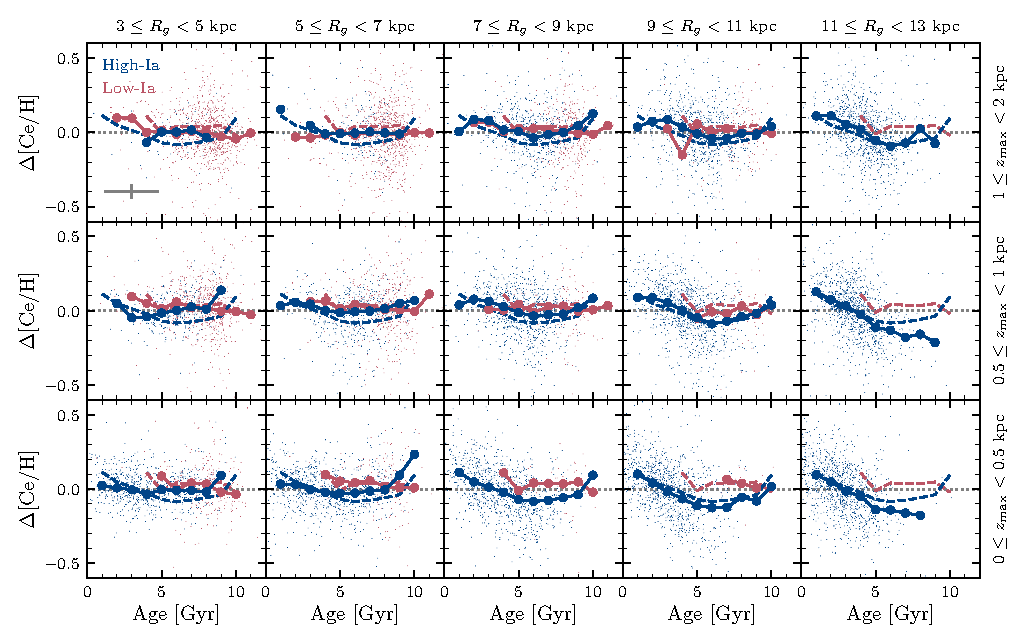
\includegraphics[width=\linewidth]{figures/residual_abundances.pdf}
%     \caption{Residual age--$\Delta$[Ce/H] trends for high- and low-Ia stars across the Galaxy.}
%     \label{fig:residual-abundances}
% \end{figure*}

\begin{figure}
    \centering
    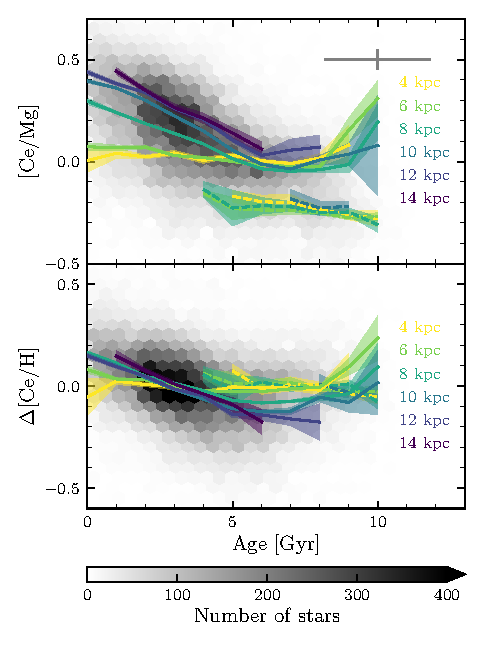
\includegraphics[width=\linewidth]{figures/median_age_trends.pdf}
    \caption{Median age trends in bins of $R_{\rm guide}$ for high-Ia (solid) and low-Ia (dashed) populations. Stars are restricted to $z_{\rm max}<0.5$ kpc.}
    \label{fig:median-age-trends}
\end{figure}

\begin{figure}
    \centering
    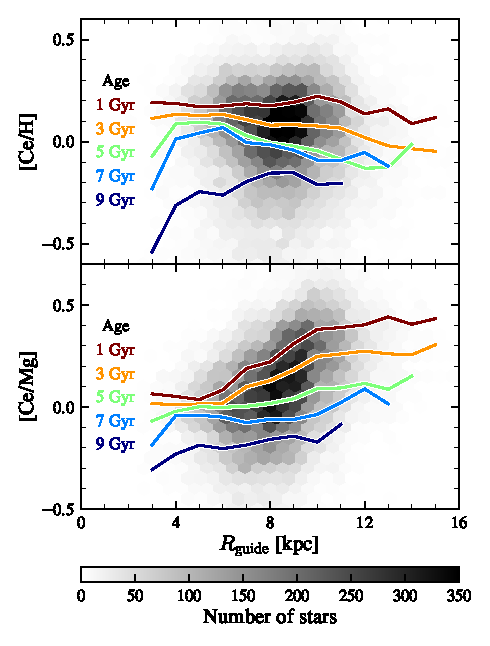
\includegraphics[width=\linewidth]{figures/ce_gradient.pdf}
    \caption{Radial gradients of [Ce/H] and [Ce/Mg] as a function of stellar age for the high-Ia (solid lines) and low-Ia subsets (dashed lines). Stars are restricted to $z_{\rm max}<0.5$ kpc.}
    \label{fig:ce-gradient}
\end{figure}

Figure \ref{fig:ce-gradient} shows the radial [Ce/H] and [Ce/Mg] gradients in bins of stellar age. Within the high-Ia subsample, the radial [Ce/H] gradient is negative with a remarkably consistent slope for $\ge5\Gyr$ old stars, whereas it is nearly flat for the youngest stars. The [Ce/Mg] gradient evolves in a similar direction, except the oldest stars show a mostly flat gradient (from $6-8\Gyr$, excluding the $9\Gyr$ bin because it contains few stars), while the youngest stars exhibit a steep {\it positive} gradient.

\subsection{The Halo}
\label{sec:halo}

\begin{figure*}
    \centering
    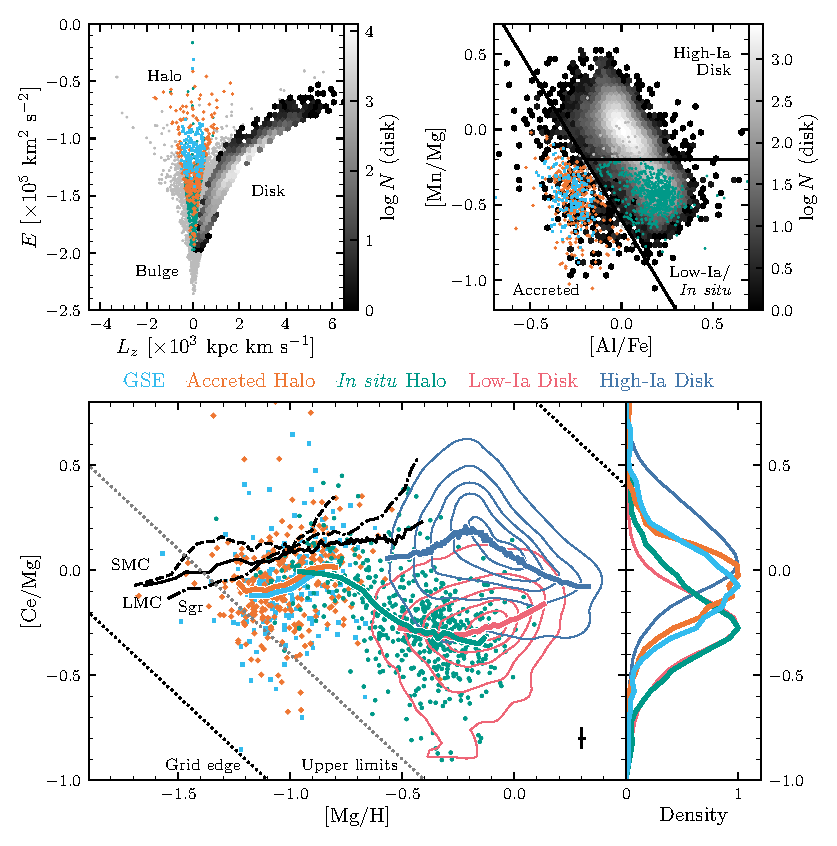
\includegraphics[width=0.8\linewidth]{figures/halo.pdf}
    \caption{{\it Top left:} Kinematic selection criteria for MW halo stars. {\it Top right:} Chemical selection criteria for accreted stars. {\it Bottom:} Ce abundance patterns for halo (green) and accreted (purple) stars as compared to the MW disk (2-D histogram). Solid lines plot a rolling median (window size 100) for the halo and accreted samples.}
    \label{fig:halo}
\end{figure*}

\section{Galactic Chemical Evolution}
\label{sec:gce}

Run the following multi-zone models (all with inside-out SFH and Gaussian migration scheme):

\begin{itemize}
    \item AGB yields only, at multiple scales. Show that AGB alone cannot match either the abundance distributions or the age relation.
    \item AGB + prompt $r$-process, using the CCSN channel. This is comparable to the \citet{grisoni_modelling_2020} models, which assume a 1 Myr delay time for all NSM. Show this does not fix the problem with the age relation.
    \item A model including a delayed NSM contribution. Hack this together using two GCE models, one of which uses the SN Ia channel for pseudo-NSM Ce enrichment, the other uses SN Ia for Fe production. Show the DTD timescale that's required to get the age relation to look like the data.
    \item Similar to above, but with radial migration cranked to 11. Does radial migration contribute to some or all of the age trend?
\end{itemize}

Additionally, using the best GCE model:

\begin{itemize}
    \item Predict age--abundance trends for $s$- and $r$-process elements not in SDSS-V.
\end{itemize}

\begin{figure}
    \centering
    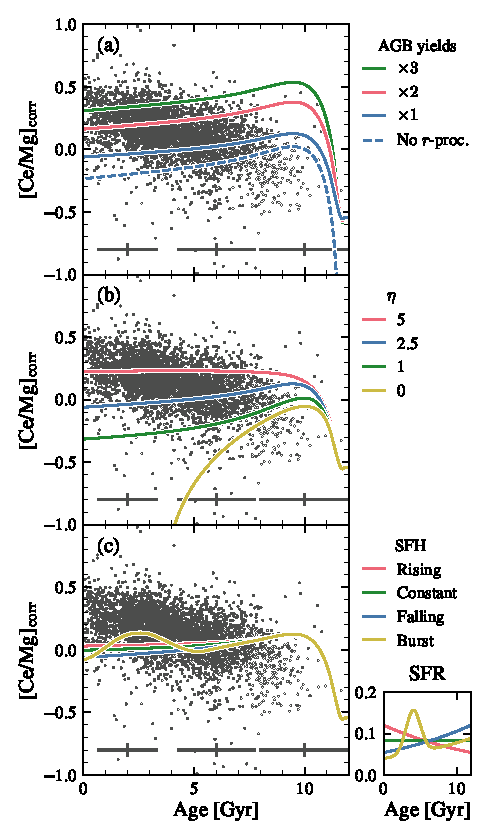
\includegraphics[width=\linewidth]{figures/agb_enrichment_models.pdf}
    \caption{The effect of adjustments to AGB yield predictions on GCE model predictions. In each panel, the gray filled (open) points are low-Ia (high-Ia) stars in the Solar neighborhood ($7\leq R_g<9\kpc$, $z_{\rm max}<0.5\kpc$) with $-0.1\leq\bracket{Mg}<+0.1$. The $\odot$ symbol marks the Solar age and [Ce/Mg], and the gray error bars represent the median uncertainties for the plotted sample. The colored curves plot the gas abundance evolution of various GCE models, with the blue curve representing the same model in each panel. {\bf (a)} Global enhancement of the AGB yields; the dashed curve is a model without a prompt Ce enrichment channel. The ``$\otimes$'' symbol represents the Solar $s$-process fraction \citep{arlandini_neutron_1999}. {\bf (b)} Multiplicative scaling of the AGB progenitor masses. {\bf (c)} Multiplicative scaling of the AGB progenitor metallicities.}
    \label{fig:agb-enrichment-models}
\end{figure}

\begin{figure}
    \centering
    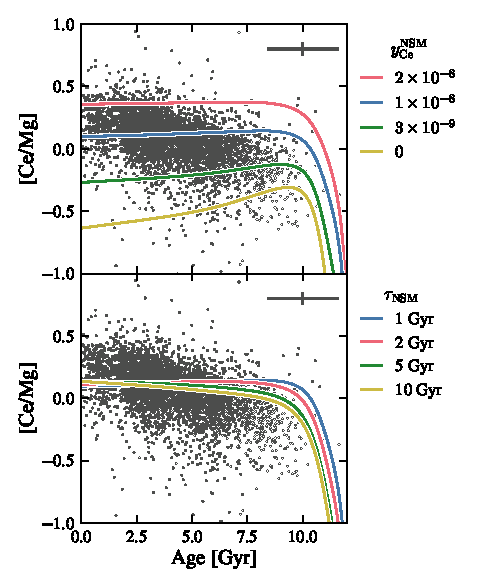
\includegraphics[width=\linewidth]{figures/delayed_enrichment_models.pdf}
    \caption{Caption}
    \label{fig:delayed-enrichment-models}
\end{figure}

\section{Conclusions}
\label{sec:conclusions}

Observational conclusions:
\begin{itemize}
    % \item Is [Ce/Mg] a true chemical clock?
    % \item What does Ce tell us about the story of the formation of the Milky Way?
    % \item (GCE modeling) What is the story of Ce itself? What does it say about the yields?
    \item Globally, stellar [Ce/Mg] ratios have a \todo{significant} negative trend with stellar age, \todo{especially for $\lesssim6\Gyr$ old stars.}
    \item The age--[Ce/Mg] relation is strongly dependent on metallicity, with the steepest trends around \todo{$0.5Z_\odot$}. The most metal-rich stars have flat age trends.
    \item The age--[Ce/Mg] relation also shows a strong dependence on galactocentric radius, even after correcting for metallicity effects. Inner galaxy stars have a flat trend with age, while outer galaxy stars show the steepest trends. Young, outer disk stars have the highest [Ce/Mg] ratios.
\end{itemize}

Model conclusions:
\begin{itemize}
    \item GCE models with standard assumptions for AGB yields predict that [Ce/Mg] should increase with stellar age, at variance with observations. \todo{A starburst can temporarily increase [Ce/Mg] ratios, but cannot match the observed duration of the trend.}
    \item Shifting Ce production to lower-mass AGB stars delays enrichment and can improve agreement with the data.
    \item \todo{A delayed $r$-process enrichment channel does not significantly improve predictions, unless the $r/s$ ratio for Ce is higher than expected.}
\end{itemize}

\section*{Acknowledgements}

% From the Center for Belonging and Social Change, https://cbsc.osu.edu/about-us/land-acknowledgement
We would like to acknowledge the land that The Ohio State University occupies is the ancestral and contemporary territory of the Shawnee, Potawatomi, Delaware, Miami, Peoria, Seneca, Wyandotte, Ojibwe and many other Indigenous peoples. Specifically, the university resides on land ceded in the 1795 Treaty of Greeneville and the forced removal of tribes through the Indian Removal Act of 1830. As a land grant institution, we want to honor the resiliency of these tribal nations and recognize the historical contexts that has and continues to affect the Indigenous peoples of this land.

\software{}

\appendix

\section{Reproducibility}
\label{app:reproducibility}

\bibliography{references}
\bibliographystyle{aasjournalv7}

\end{document}
